%%%%%%%%%%%%%%%%%%%%%%%%%%%%%%%%%%%%%%%%%%%%%%%%%%%%%%%%%%%%%%%%%%%%%%%%%%%%%%%%
%2345678901234567890123456789012345678901234567890123456789012345678901234567890
%        1         2         3         4         5         6         7         8

%\documentclass[letterpaper, 10 pt, conference]{ieeeconf}  % Comment this lineout
                                                          % if you need a4paper
%\documentclass[a4paper, 10pt, conference]{ieeeconf}      % Use this line for a4

\documentclass[runningheads,a4paper]{llncs}

\usepackage{amssymb}
\setcounter{tocdepth}{3}
\usepackage{graphicx}
\usepackage{hyperref}

\usepackage{subfigure}

\usepackage{url}
\title{\LARGE \bf
Software Architecture
}

\begin{document}

\maketitle
\thispagestyle{empty}
\pagestyle{empty}

%%%%%%%%%%%%%%%%%%%%%%%%%%%%%%%%%%%%%%%%%%%%%%%%%%%%%%%%%%%%%%%%%%%%%%%%%%%%%%%%
\section{Introduction}

In this section, we explain the overall software architecture that we've developed for object interactions. Each module is responsible for effectively processing the information acquired from sensory-motor data streams and interaction experiences by utilizing ROS \cite{ros} and YARP \cite{yarp} at the very core of the system. A simplified and slightly modified -due to space constraints- snapshot of ROS computation graph is given in figure \ref{fig:rxgraph}, acquired via \emph{rxgraph} ROS comand-line tool.

\begin{figure}[htp]
\centering
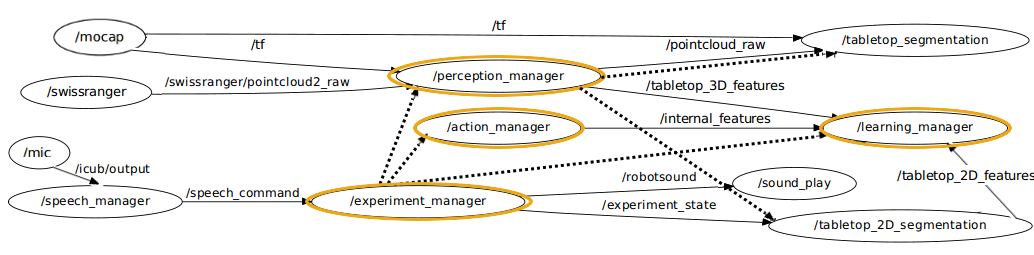
\includegraphics[width=130mm]{imgs/rx7.png}
\caption{ROS communication graph. Ellipses show the ROS nodes that are dedicated to distinct tasks. Main modules are shown in orange ellipses for reader's convenience. Dotted lines show service calls (request-response type bi-directional communication interface) and regular lines show one-way message passings between different nodes. }
\label{fig:rxgraph}
\end{figure}

We can investigate the system in four main modules; perception, action, learning, and experiment.

\subsection{Perception Module}

We have used various internal and external sensors to extract perceptual information from the environment. External sensors are Swissranger SR4000 (swissranger) time-of-flight range camera, Phoenix Technologies VisualEyez II motion capture system (mocap), and a microphone. Internal sensors are the arm and head motor encoders, hand tactile sensors, and eye cameras.

Below we explain the sub-modules that are responsible for processing the information obtained from each sensor.

\subsubsection{Tabletop 3D object segmentation and identification\newline\newline}

iCub's interaction workspace is assumed to be dominated by a planar table. It is also assumed that the interaction objects lie on the table, any other object that doesn't touch to the table is discarded during the filtering processes explained below. In order to apply diverse actions on the objects, it is necessary to recognize them to some level. Since our main focus is not about object recognition, we stopped at the point where objects are identified in terms of their bounding boxes and distinct object id labels. For this purpose, we have used several ROS packages as they are briefly explained below:

\begin{itemize}
 \item \emph{PCL}\cite{pcl} to pre-process the point cloud data obtained from swissranger sensor to filter out noisy points, and remove the points that lie outside a volume of interest (interaction workspace) which is assumed to be containing a planar table.
 \item \emph{tf} ROS package to obtain homogenous coordinate transformations between iCub and swissranger sensor based on the mocap readings.
 \item \emph{tabletop\_object\_detector} ROS package to detect the table, and cluster the 3D points on top of this plane into euclidean clusters that correspond to the table-top objects. Then, we identify the objects and index them with a simple heuristic that utilizes the position and bounding box volume information.
 \item \emph{rviz} ROS package to visualize interaction workspace and other relevant information.
\end{itemize}

Swissranger provides distance, confidence, amplitude and point cloud information as they are shown in figure \ref{fig:sr4k_data}, captured during an experiment.

\begin{figure}
\centering
\mbox{\subfigure{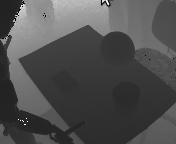
\includegraphics[width=40mm]{imgs/distance.png}}\quad
\subfigure{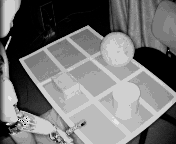
\includegraphics[width=40mm]{imgs/confidence_.png}}\quad
\subfigure{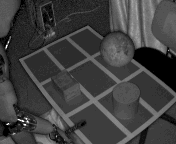
\includegraphics[width=40mm]{imgs/amplitude_.png}}}
\caption{From left to right; distance, confidence and amplitude images obtained from swissranger.} \label{fig:sr4k_data}
\end{figure}

After obtaining the raw point cloud, we do the following operations to obtain tabletop objects:
\begin{itemize}
 \item filtering out outlier points around the edges by using radius outlier removal, and filtering out non-workspace points by using three passthrough filters to specify a volume of interest in three cartesian axis which improves the overall 3D perception performance. Figure \ref{fig:filtered_3d_data} shows the filtering results.
 \item RANSAC based table detection, obtaining euclidean clusters, figure \ref{fig:clusters}
 \item object id assignment considering their volumes and positions, figure \ref{fig:ids}
\end{itemize}

\begin{figure}[ht]
\begin{minipage}[b]{0.5\linewidth}
\centering
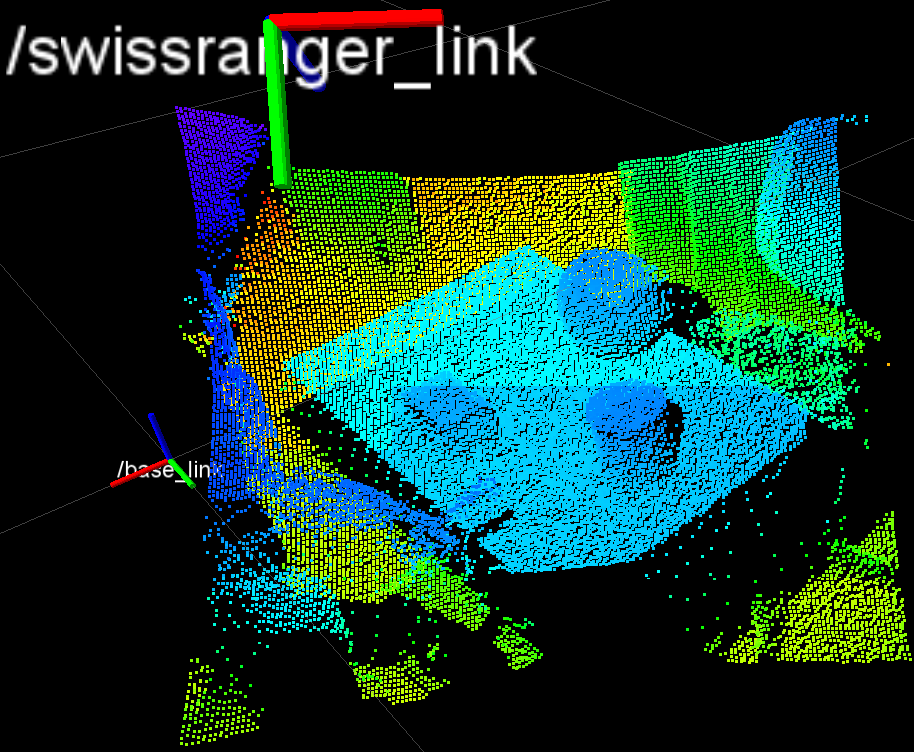
\includegraphics[width=60mm]{imgs/0.png}
\caption{Raw input point cloud.}
\label{fig:figure1}
\end{minipage}
\hspace{0.5cm}
\begin{minipage}[b]{0.5\linewidth}
\centering
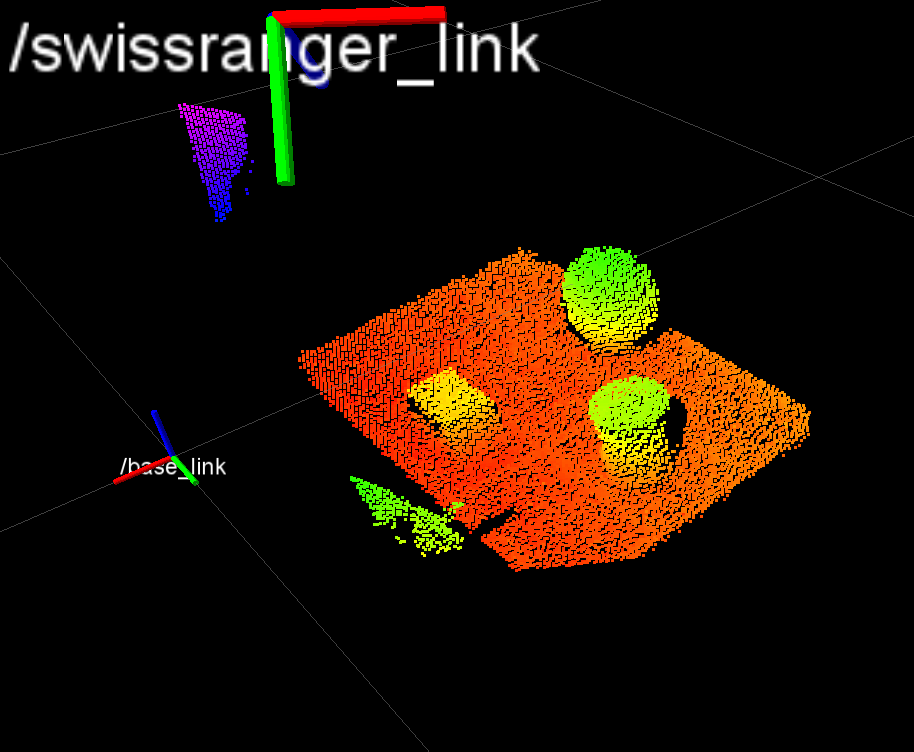
\includegraphics[width=60mm]{imgs/1.png}
\caption{Filtered point cloud}
\label{fig:filtered_3d_data}
\end{minipage}
\end{figure}

\begin{figure}[ht]
\begin{minipage}[b]{0.5\linewidth}
\centering
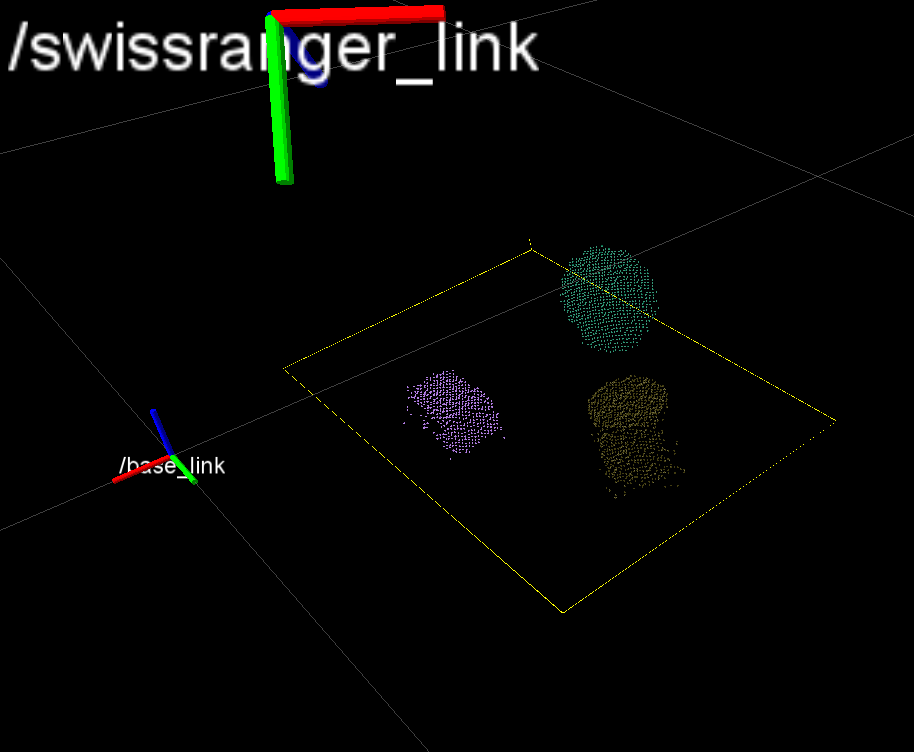
\includegraphics[width=60mm]{imgs/2.png}
\caption{Table detection, euclidean clusters.}
\label{fig:clusters}
\end{minipage}
\hspace{0.5cm}
\begin{minipage}[b]{0.5\linewidth}
\centering
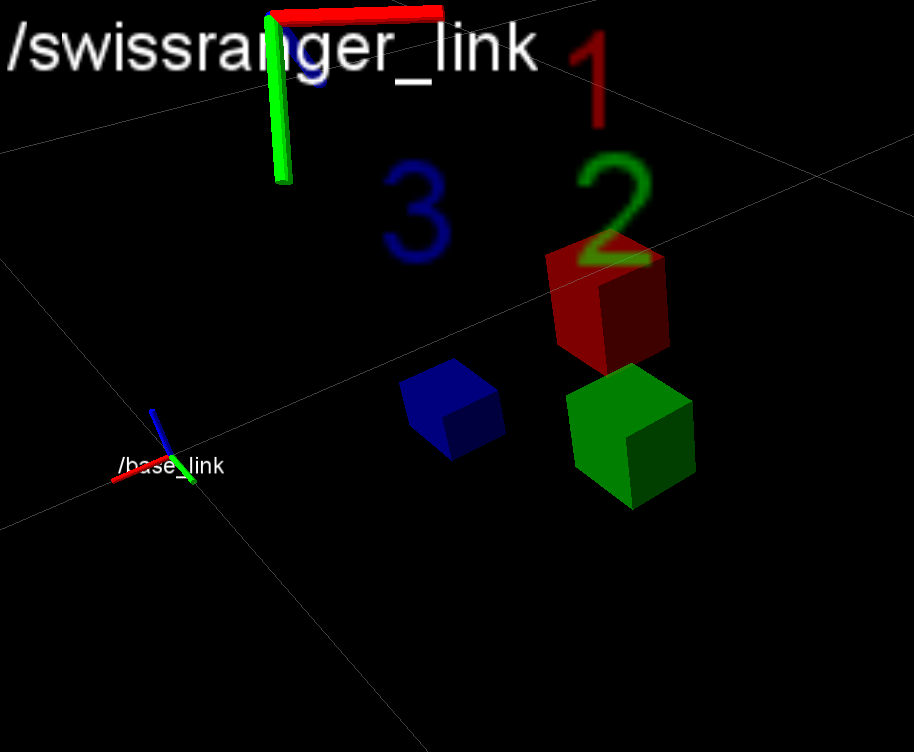
\includegraphics[width=60mm]{imgs/4.png}
\caption{Object id assignment}
\label{fig:ids}
\end{minipage}
\end{figure}

\subsubsection{Tabletop 2D object segmentation and identification\newline\newline}

Experiments consist of interactions between different sized, colored objects and iCub on the experiment table. Experiment table is prepared on a black background with nine equal sized regions determined with white borders in order to simplify the image processing. Segmentation process of the objects on the experiment table is crucial for iCub to extract the necessary features for the learning process of the actions. To extract features for learning process, a few image processing operations are required on the images from eyes. These processes are given below:
\begin{itemize}
 \item \emph{Extracting Corner and Edge Features: } In order to find the region edges, binary threshold is applied on image and on this binary image, OpenCV's \cite{opencv} feature extraction function is used. Figure \ref{fig:Extracting Corner and Edge Features} shows these processed images.
\begin{figure}
\centering
\mbox{\subfigure{
\includegraphics[width=60mm]{imgs/edges.png}}\quad
\subfigure{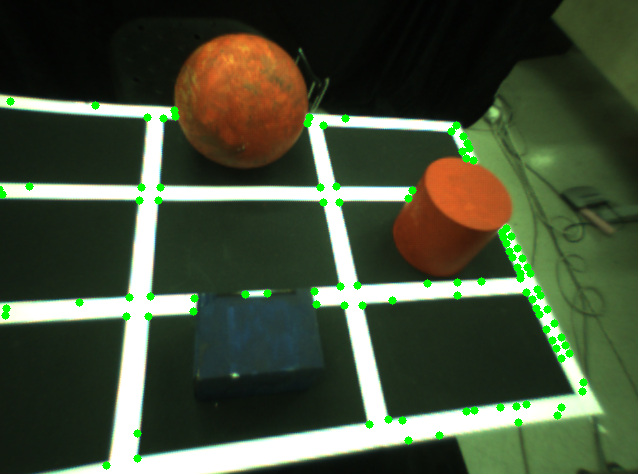
\includegraphics[width=60mm]{imgs/allfeatures.png}}}
\caption{Left part of the figure is the binary thresholded input image, right one is the extracted features using OpenCV} \label{fig:Extracting Corner and Edge Features}
\end{figure}
 \item \emph{Verification and Identification of Region Corners and Regions: } Among the extracted features, a few of them are qualified as real region corners after verification. Then on percepted image, depending on interval and extension colors between corners, these corners are labeled thereby regions which can be seen in Figure \ref{fig:Verification and Identification of Region Corners and Regions}.
\begin{figure}
\centering
\mbox{\subfigure{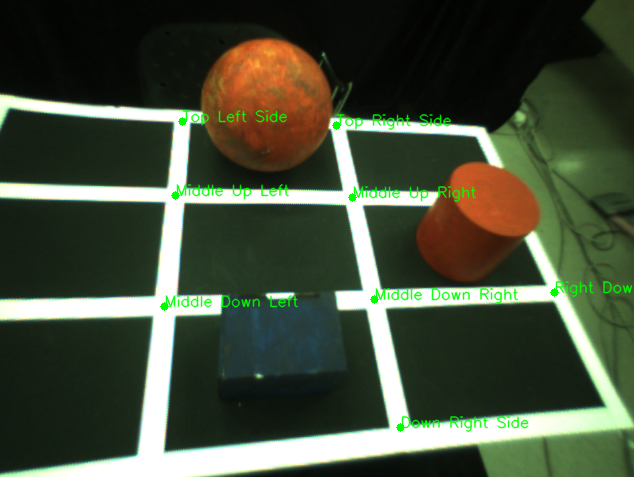
\includegraphics[width=60mm]{imgs/cornersIdentified.png}}\quad
\subfigure{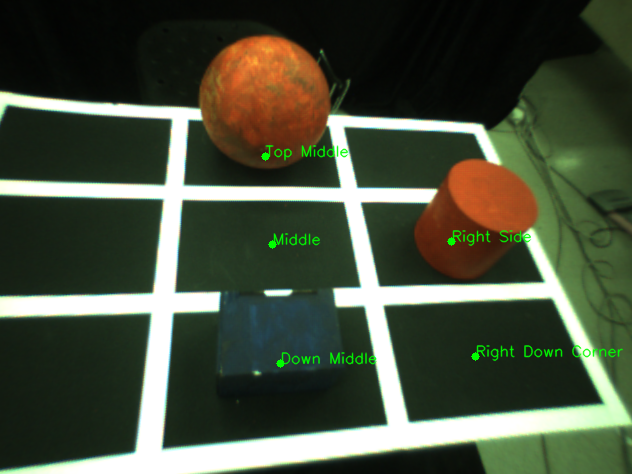
\includegraphics[width=60mm]{imgs/regions.png}}}
\caption{Left part of the figure is the verified and identified region corners and right part is the regions determined by region corners } \label{fig:Verification and Identification of Region Corners and Regions}
\end{figure}
 \item \emph{Hue Channel Thresholding and Segmentation: } Percepted BGR image is converted into HSV image type and its hue channel is retrieved. On this channel, image is thresholded in some range to get rid of background color and as keeping images visible as can be seen in Figure \ref{fig:Hue Channel Thresholding and Segmentation}. Since 2D region coordinates are known, OpenCV's flood fill function is used to get segmented object from known coordinates. 
 \item \emph{Face Detection: }When iCub raises his head and reached a threshold, OpenCV's face detection algorithm takes place in order to detect human presence in the experiments.
 \item \emph{Visualization of Segmented Objects and Face on Wireframe: } Since regions and objects in these regions are known, these segmented objects are shown like in Figure \ref{fig:Visualization of Segmented Objects and Face on Wireframe} on a table wireframe with a detected face above it, if human presence is detected  
\begin{figure}[ht]
\begin{minipage}[b]{0.5\linewidth}
\centering
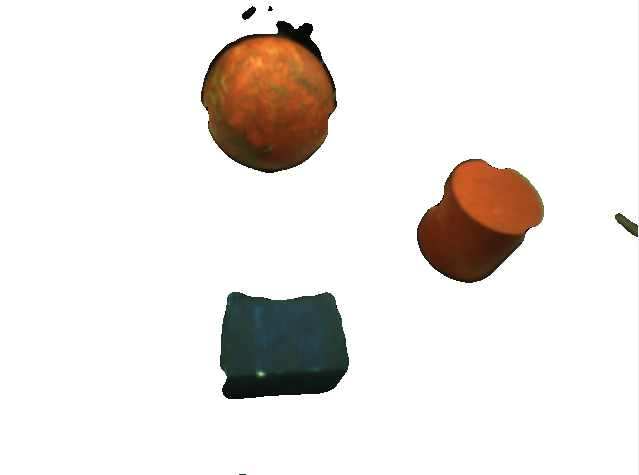
\includegraphics[width=70mm]{imgs/filteredImage.png}
\caption{Segmented Objects.}
\label{fig:Hue Channel Thresholding and Segmentation}
\end{minipage}
\hspace{0.5cm}
\begin{minipage}[b]{0.5\linewidth}
\centering
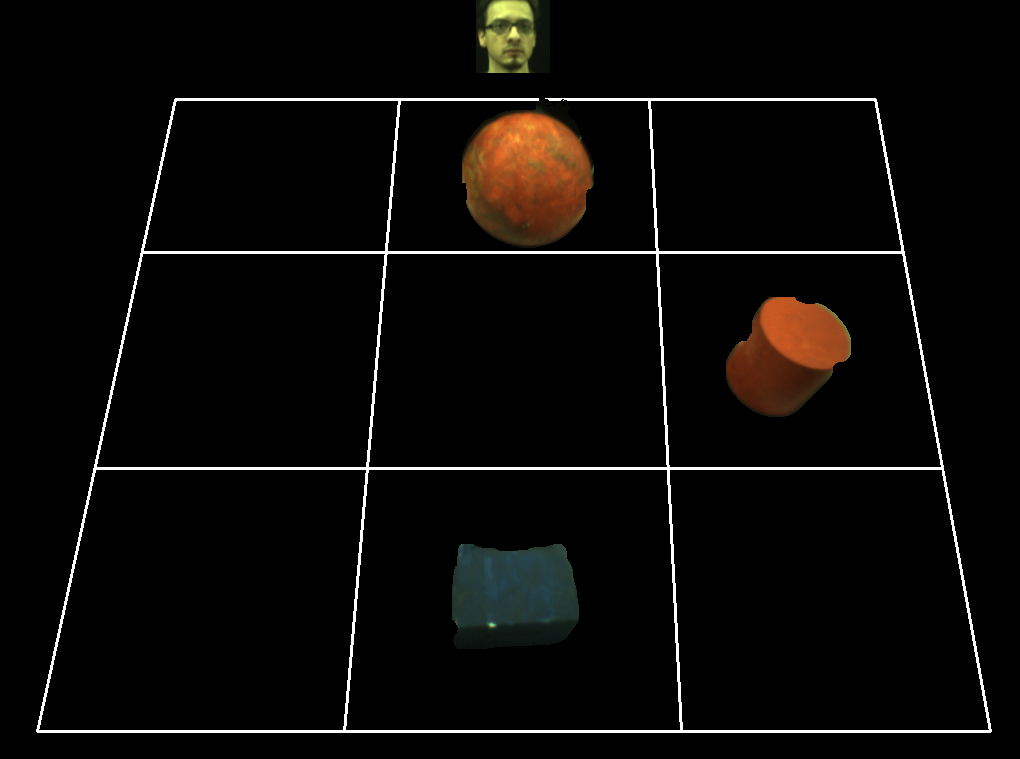
\includegraphics[width=70mm]{imgs/wireframeLast.png}
\caption{Visualization of Segmented Objects and Face on Wireframe }
\label{fig:Visualization of Segmented Objects and Face on Wireframe}
\end{minipage}
\end{figure}
\end{itemize}

\subsubsection{Feature Extraction and Visualization}

After 2D and 3D object segmentation and identification sub-modules are finished, a feature vector is retrieved for learning module. This feature vector is given below: \\
\[
f_{perceptual} =
\left[ {\begin{array}{cc}
{human\_presence} \\
{object\_ROI\_position (x, y)} \\
{object\_ROI\_size (width, height)} \\
{object\_area} \\
{[object\_red\_color\_histogram\_10\_bin]} \\
{[object\_green\_color\_histogram\_10\_bin]} \\
{[object\_blue\_color\_histogram\_10\_bin]} \\
{[surface\_normal\_azimuth\_20\_bin]} \\
{[surface\_normal\_zenith\_20\_bin]} \\
{bounding\_box\_position (x, y, z)} \\
{bounding\_box\_volume} \\
\end{array} } \right]
\]				      

\begin{figure}[ht]
\begin{minipage}[b]{0.5\linewidth}
\centering
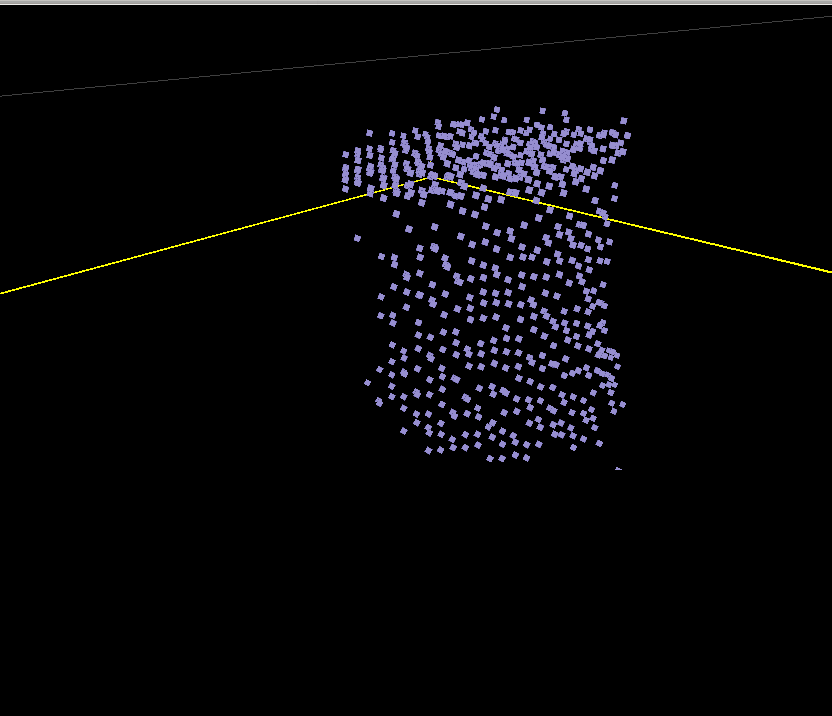
\includegraphics[width=60mm]{imgs/object_cluster.png}
\caption{Clustered object.}
\label{fig:ids}
\end{minipage}
\hspace{0.5cm}
\begin{minipage}[b]{0.5\linewidth}
\centering
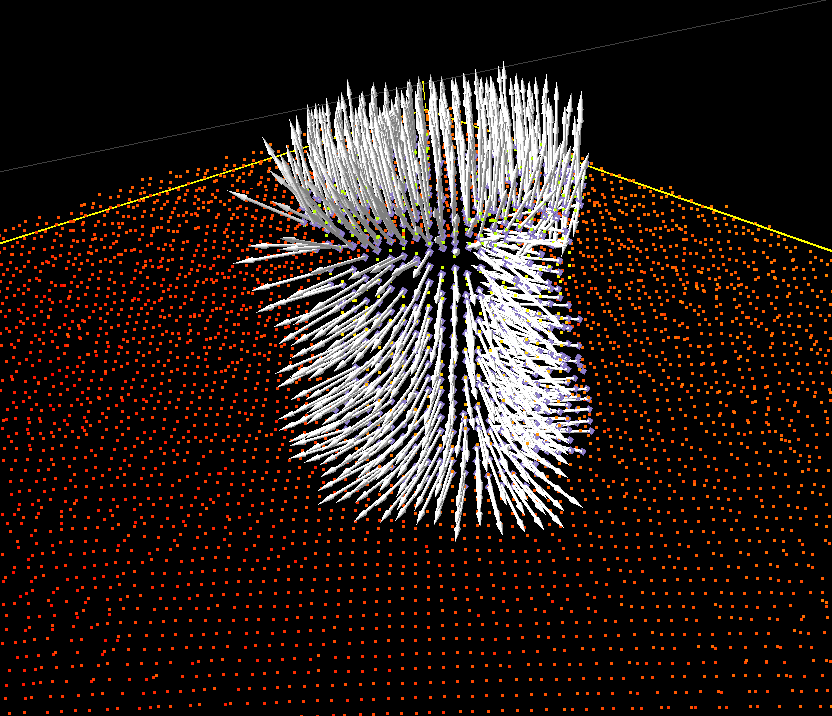
\includegraphics[width=60mm]{imgs/surface_normals.png}
\caption{Surface normal estimation. }
\label{fig:rxgraph}
\end{minipage}
\end{figure}

Surface normal histogram values of this cylindrical object is given as follows:

\begin{figure}[ht]
\centering
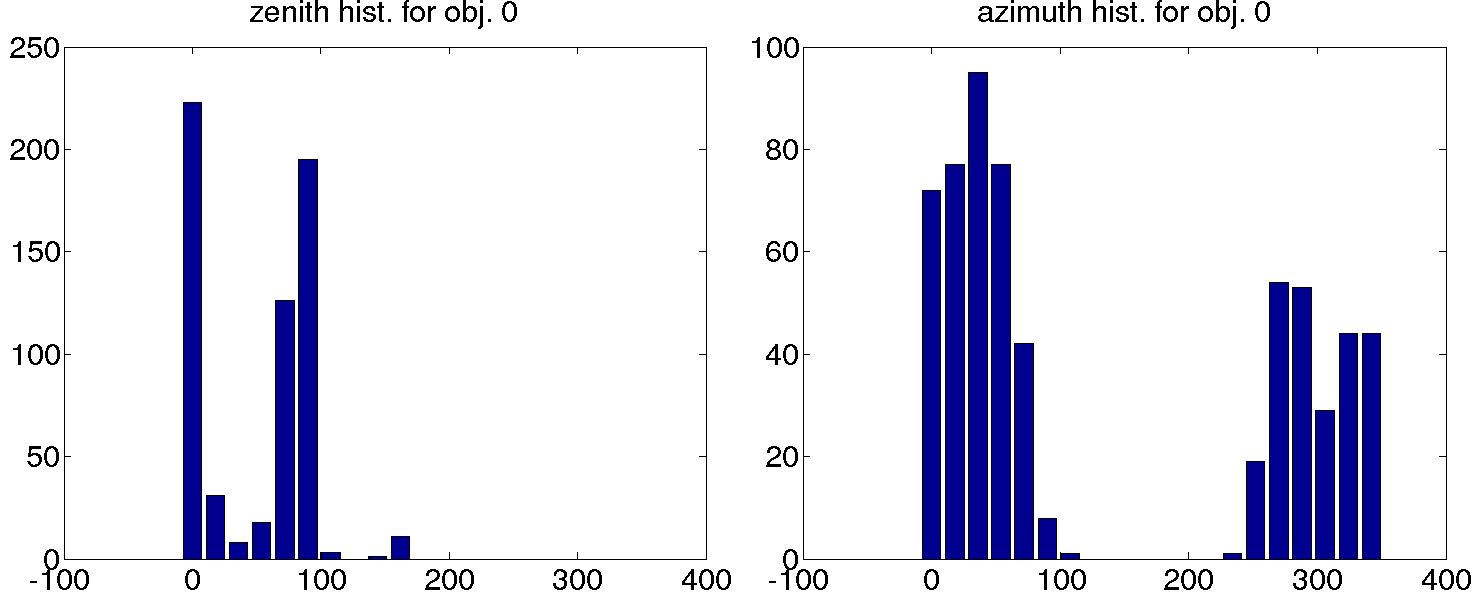
\includegraphics[width=140mm]{imgs/untitled.png}
\caption{Azimuth and zenith angle histograms }
\label{fig:rxgraph}
\end{figure}

Surface color histograms are shown below:

\begin{figure}[ht]
\centering
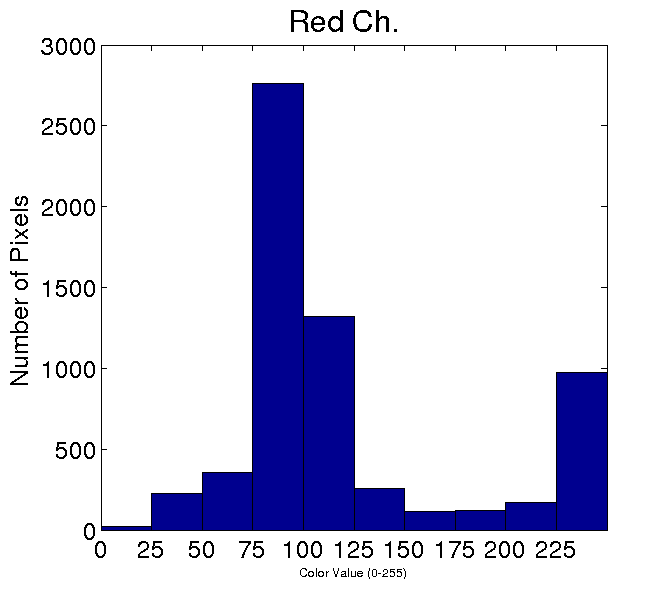
\includegraphics[width=70mm]{imgs/red.png}
\caption{Azimuth and zenith angle histograms }
\label{fig:rxgraph}
\end{figure}

\begin{figure}[ht]
\centering
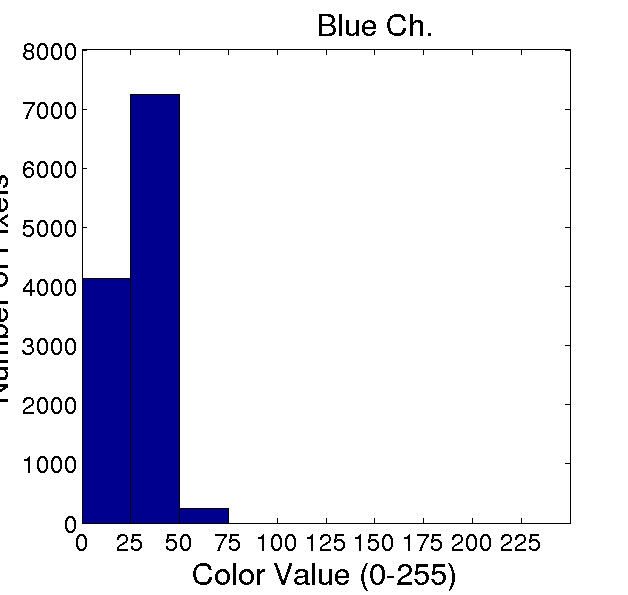
\includegraphics[width=70mm]{imgs/blue.png}
\caption{Azimuth and zenith angle histograms }
\label{fig:rxgraph}
\end{figure}

\begin{figure}[ht]
\centering
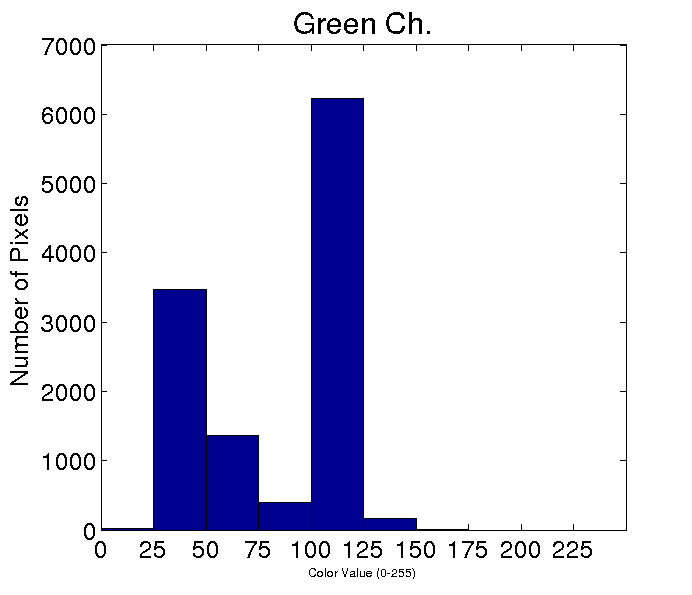
\includegraphics[width=70mm]{imgs/green.png}
\caption{Azimuth and zenith angle histograms }
\label{fig:rxgraph}
\end{figure}

\subsection{Action Module}

We have developed this module on top of iCub \emph{actionPrimitives} library, by extending its basic functionalities. This module enables iCub to apply push, grasp, show, look, hide, take, give, reach, basket, and other similar actions. This module is also responsible for extracting features related to the action experiences. These features include end-effector position, tactile sensor data on each finger, and the palm.

\[
f_{internal} =
\left[ {\begin{array}{cc}
head\_joint\_angles (j_0, j_1, j_2)\\
torso\_joint\_angles (j_0, j_1, j_2)\\
end\_effector\_position (x,y,z)\\
\end{array} } \right]
\]	

\subsection{Learning Module}

This module subscribes to the other modules (through ROS network) to gather feature and label information. This information is used to learn affordances, or predict learned affordances based on an SVM learner, \cite{svm}. Weka's \cite{weka} ReliefF algorithm implementation is used to extract relevant features from the main feature vector.

\subsection{Experiment Module}

This module is the main control center of the system. It makes service calls to other modules and manages the sensory-motor data communication between modules. It is also the human-robot acoustic communication interface which manages the service calls to speech recognizer and speech synthesizer modules. We use \emph{pocketshpinx} ROS package as the speech recognizer which wraps around CMU pocket shpinx\cite{sphinx}, and \emph{audio\_common} ROS package as the speech synthesizer that utilizes festival speech synthesis system \cite{festival}.

A sample experiment script is given below:
\begin{itemize}
\item iCub: \emph{``Please tell me what to do!''} ( iCub asks for an action from it's action reportiore to apply.)
\item Human: \emph{``iCub push left object one''}  ( Human directs iCub to apply push left action on an object that is labeled as \emph{one}. Human knows this label by looking at an \emph{rviz} window shown on one of the test-setup monitors.)
\item iCub: \emph{``I'm percepting...''} ( iCub acknowledges human that it is extracting perceptual features before applying any action)
\item iCub: \emph{``I guess object one is going to be vanished''} (iCub predicts the effect before applying the specified action based on the svm models it already learned.)
\item iCub: \emph{``I'm pushling left object one''} (iCub extracts internal features (proprioceptive and tactile) just before applying the action to the object)
\item iCub: \emph{``Please tell me what happened''} (iCub asks for the effect id to store this experiment data for future learning procedures.)
\item Human:\emph{``iCub object one is disappeared''} (Human supervises iCub about the effect it has generated on this particular object.)
\end{itemize}

\begin{thebibliography}{99}

\bibitem{ros}
M. Quigley, K. Conley, B. Gerkey, J. Faust, T. B. Foote, J. Leibs, R. Wheeler, and A. Y. Ng, "ROS: an open-source Robot Operating System," in ICRA workshop on Open-Source Software, 2009.

\bibitem{yarp}
G. Metta, P. Fitzpatrick \& L. Natale. YARP: Yet Another Robot Platform. International Journal on Advanced Robotics Systems, 3(1):43--48, 2006.

\bibitem{pcl}
Rusu, Radu Bogdan; Cousins, Steve; , "3D is here: Point Cloud Library (PCL)," Robotics and Automation (ICRA), 2011 IEEE International Conference on , vol., no., pp.1-4, 9-13 May 2011
doi: 10.1109/ICRA.2011.5980567 

\bibitem{opencv}
G. Bradski and A. Kaehler, Learning OpenCV: Computer Vision with the OpenCV Library. O'Reilly Media, Inc., 2008, pp. 415-453

\bibitem{svm}
C.-C. Chang and C.-J. Lin. LIBSVM : a library for support vector machines. ACM Transactions on Intelligent Systems and Technology, 2:27:1--27:27, 2011.

\bibitem{weka}
Mark Hall, Eibe Frank, Geoffrey Holmes, Bernhard Pfahringer, Peter Reutemann, Ian H. Witten (2009); The WEKA Data Mining Software: An Update; SIGKDD Explorations, Volume 11, Issue 1.

\bibitem{sphinx}
Willie Walker, Paul Lamere, Philip Kwok, Bhiksha Raj, Rita Singh, Evandro Gouvea, Peter Wolf, and Joe Woelfel. 2004. Sphinx-4: A Flexible Open Source Framework for Speech Recognition. Technical Report. Sun Microsystems, Inc., Mountain View, CA, USA.

\bibitem{festival}
A.W. Black, P. Taylor, and R. Caley, “The festival speech synthesis system,” http://www.festvox.org/festival/

\end{thebibliography}

\end{document}
